\documentclass[final,3p,twocolumn,authoryear,sort&compress,times]{maia}
%\documentclass[final,1p,authoryear,sort&compress,times]{maia}
\journal{MAIA Master}


%% PACKAGES %%%%%%%%%%%%
% Add as packages as necessary
\usepackage{amsmath,amssymb}	
\usepackage{graphicx}
\usepackage{hhline}	
\usepackage{color}
\usepackage{natbib}
\usepackage{hyperref}
\usepackage{float}
\usepackage{algorithm}
\usepackage{algorithmic}
\usepackage{multirow}
\usepackage{hyperref}
%% BIBLIOGRAPHY %%%%%%%%
% MAIA bibliography style
\bibliographystyle{model2-names}

%% Definitions %%%%%%%%%
% Add as new commands as necessary
\definecolor{red}{RGB}{255,0,0}
\newcommand{\aobf}[1]{\textbf{\color{red} #1}}

\graphicspath{{./}{./figures/}}

% \hypersetup{draft}
\begin{document}

\begin{frontmatter}

%name of the thesis
\title{GAN (Generative Adversarial Networks) for realistic data augmentation and lesion simulation in x-ray breast imaging}

\fancyhead[LO]{GAN for realistic data augmentation and lesion simulation in x-ray breast imaging}
%%authors (choose one of the options)
%option 1 => Only student name
%\author{Student Name}
%\address{Adress of the Student}
%option 2 => Student and Supervisor(s) name with same affiliation
\author{Basel Alyafi, \textbf{Supervisors: }Robert Marti, Oliver Diaz}
\address{Universitat de Girona, 17003, Girona, Spain}
%option 3 => Student and Supervisor(s) name, different affiliation
%\author[addressStudent]{Student Name}
%\author[addressSupervisor]{Supervisor Name}
%\address[addressStudent]{Adress of the Student}
%\address[addressSupervisor]{Address of the Supervisor, if different}

\begin{abstract}
Early detection of breast cancer has a major contribution to curability, and this importance increases when using non-invasive solutions as mammographic images. Supervised deep learning methods have played a great role in object detection in computer vision, but it suffers from a limiting property; the need to huge labelled data. This becomes stricter when it comes to medical datasets which have high-cost time-consuming annotations. As a leveraging method, Deep Convolutional Generative Adversarial Networks (DCGANs) are proposed here to ameliorate this problem, they are trained on different-size partial subsets of one dataset and used to generate diverse and realistic mammographic lesions. The effect of adding these images is tested in an environment where a 1-to-10 imbalanced dataset of lesions and normal tissue is classified by a fully-convolutional neural network. We show that using the synthetic images in this environment outperforms the traditional augmentation method of flipping. A maximum of $\sim0.09$ and $\sim0.013$ improvement of F1 score and AUC, respectively, were reported by using GANs along with flipping augmentation compared to using the original images even with relatively-small dataset sizes. We show that DCGANs can be used for synthesizing photo-realistic mammographic mass patches with a considerable diversity measured using Frechet Inception Distance (FID). 
%These synthetic patches were shown using t-distribution Stochastic Neighbor Embedding (t-SNE) to have a distribution that can help in classification problems.
\end{abstract}

\begin{keyword}
computer-aided detection \sep generative adversarial networks \sep data augmentation \sep breast cancer \sep deep learning  \sep fully-convolutional neural networks \sep t-Stochastic Neighbor Embedding.
\end{keyword}

\end{frontmatter}


\section{Introduction}
\label{sec:introduction}
    \subsection{Breast Cancer Detection}
Cancerous breast cells have been the second deadliest disease in women globally coming after lung cancer. This disease was the most frequently diagnosed cancer in 154 countries and the first cause of cancer death in women in 100 countries in 2018 \citep{cancer_stats}. In EU, breast cancer was the first cause of cancer death in 2014 for women, while for men it was lung cancer. Approximately, over 92000 women are anticipated to die because of breast cancer in 2019 with a similar number of deaths in 2014 \citep{EU_stats}. Computer-aided detection (CADe) systems have shown that they can assist specialists in decision making although recent studies show that patient recalls have increased when using artificial intelligence as a second reader \citep{ai_breastImaging}. Moreover, CADe systems have been a good alternative for double reading to reduce failures resulted from mainly: visual search mistakes due to fatigue or other reasons, and mistakes in interpretation due to lack of decision-making experience for inexperienced interpreters \citep{Bazzocchi2007}. These systems can help reduce the diagnostic accuracy differences between radiologists caused by intra- and inter-observer variability \citep{radiologists_variability}. Particularly, these systems can increase the sensitivity of less-experienced interpreters by increasing the detection rate by 10\% (as a maximum) and reducing the time needed to detect the disease by one month in the best case. That said, the benefits observed in more-experienced readers is much smaller \citep{CAD_failed}. Additionally, CADe systems, represented currently by neural networks, require large amounts of annotated data when using supervised learning. Unsupervised learning is still under research where there is no need for completely-labelled datasets. However, a large number of experiments is usually needed to teach the system making deep learning in general a limited-capability tool if the need to a large enough data is not met properly. Furthermore, publicly-available medical datasets are usually small and imbalanced due to concerns mainly related to privacy and  the high costs needed to produce professional annotations by experts. To alleviate this problem of lack of data, different methods ranging from conventional data augmentation using affine transformations such as flipping or scaling, passing by sampling methods, to the more effective but complex way using Generative Adversarial Networks (GANs) \citep{GAN}.

\subsection{Generative Adversarial Networks}
\label{sec:GAN}

To use machine learning tools in CADe systems, a reasonable amount of medical data is needed to train the system on capturing abnormalities in input images that specialists try to detect. These abnormalities differ from one medical field to another, breast lesions and lung nodules, for instance. Public medical datasets usually suffer from unbalanced distribution of images between the classes under study. Target class images are commonly rare, for example in INbreast dataset, by \citet{INbreast}, one fourth of the dataset contains breast lesions. Intrinsically, in a mammographic image, normal tissue patches largely outnumber lesion patches (the target concept), if there is any, when classifying with/without lesion images patch wise. When this kind of problem exists, the learning process becomes more difficult and sometimes might lead to a loss in generalisation (overfitting). To overcome this obstacle, scholars usually use different methods: oversampling the weak class (e.g. \textit{SMOTE} and \textit{ADASYN}), undersampling the strong class, or ensembling the weak class with subsets of the strong class to make multiple smaller balanced datasets (for instance \textit{Easy Ensemble}, \textit{BestCascade} and \textit{NearMiss}) \citep{imbalanced_learning}. Most oversampling methods, if not all, in general, use either samples replication, interpolation, or extrapolation. By replication, the algorithm tries to push the population up by replicating some samples identically. Interpolation-based methods insert new samples that are derived from the neighbourhood by averaging the features, i.e., averaging two neighbouring samples belonging to the same class to find the midpoint sample. Finally, extrapolation methods, as image rotation, translation, and zooming, produce new samples that can increase the generalisation of the model by reducing (or removing) the contribution of some sorts of non-pertinent variance--differences that are unrelated to the discrimination process--in properties like image angle, center position, and size to decision making \citep{GAN_brain_aug}. However, not all non-pertinent information is as easy to exclude from discriminative features as affine transformations, especially in medical imaging field where there is a lack of conventional augmentation tools to tackle all sources of non-pertinent variance. %Generative models P2P, Boltzman machines 
GANs, introduced in \citet{GAN}, made a revolution in the field of data synthesisation, where a network (called generator or G) learns the distribution of the input data implicitly by the aid of another network (called discriminator or D) which, in turns, tries to learn to distinguish real among fake (synthetically-generated) images and feed the result back to G to update the weights. In other words, G learns the mapping $Z \to X$, where Z is the latent space (noise) and X is the data distribution, while D learns the mapping $X \to [0,1]$. These two networks learn simultaneously in order to get in the end a generator that can yield realistic and diverse images starting from a random input (latent vector). In theory, when the generator and discriminator become experts, G generates images that are classified as well as real images with a probability of 0.5, which is known as Nash equilibrium. To reach near this point, the learning process should converge in such a way that neither G nor D learns in a pace that is much higher than the other. Furthermore, GANs have the big advantage of being able to augment a wide range of variance sources providing that the dataset has enough examples. As an example, consider a breast mass detection problem where micro calcifications should not affect the decision, by applying traditional methods of augmentation it is hardly ever possible to add calcification to a mass-only lesion which can be done using a trained generator.
Two main problems might come up when training GANs \citep{nips2016}:
\begin{itemize}
    \item Mode collapse: this happens when the network generates images that are replications of one pattern with slight differences. In this case, G has a many-to-one mapping between the latent space and the output images. As a consequence, the diversity of the outputs will be low (low recall) while realism might be fine. In multi-class problems, two kinds of mode collapse (or equivalently mode dropping) might exist: intra-class and inter-class, where in the former kind, the generator synthesises images for which the per-class diversity is low, while, in the latter kind, G synthesises images from one (or a few) class(es) only, ignoring others.
    \item Oscillation: when the generator keeps generating different samples but with low realism (low precision) which are easy for D to reject. Meaning that the system never converges, this is commonly caused by imperfect tuning for the learning speed of G and D, where D learns quickly giving no time for G to improve. This results in G loss increasing early in the training process while D loss reaches low values.

\end{itemize}
In this paper, Deep Convolutional GAN (DCGAN) was selected due to training stability as presented in \citet{radford_DCGAN}. It was used to synthesise mammographic lesions to use them as data augmentation to support CADe for breast mass detection.
The rest of this paper is organised as follows: section \ref{sec:stateoftheart} describes in brief recent works on GANs in medical imaging. Materials are explained in section \ref{sec:dataset}, while methods are presented in section \ref{sec:gan_arch_train}. Sections \ref{sec:results}, \ref{sec:discussion}, and \ref{sec:conclusions} include the results, discussion and conclusions, respectively.
The contributions of this work are as follows:
\begin{enumerate}
    \item We show that DCGANs are able to generate images of $128 \times 128$ pixels of realistic and diverse mammographic mass and calcification lesions evaluated quantitatively using Frechet Inception Distance.
    \item We tested the DCGANs performance after being trained and we show that it provides remarkable improvements when used to augment an imbalanced dataset.
    \item We analysed the effect of adding the synthesized images to an imbalanced dataset as a function of training set size in a classification problem.
     \item We propose one framework (Figure \ref{fig:methodology}) under which all previous points can be tested combined using 3-fold cross validation.
     \item We show that the generated images belong to the real images' distribution by visualizing the t-Stochastic Neighbor Embedding (t-SNE) of both real and fake images.
     \item We made the trained generators publicly available, along with the code, to the scientific community to generate patches of breast masses.
\end{enumerate}


\section{State of the art}
\label{sec:stateoftheart}
\citet{highresol_mammoGAN} used Progressive GANs to generate 1280 $\times$ 1024 full mammogram images that show breast anatomy with acceptable amount of fine details using the multi-stage adversarial learning introduced in \citep{progressive_GAN}. In \citet{lung_GANs}, 5-class chest pathology X-ray $256 \times 256$ images were generated using the well-known DCGAN architecture by \citet{radford_DCGAN}. They evaluated the effect of including the synthesized images by measuring the balanced test accuracy using three models, namely: real imbalanced dataset (DS1), real balanced dataset (DS2) with 2K images from each class, and balanced real + synthesized images (DS3) with approximately 30K images from each class. The results clearly showed that including synthetic images boosted the performance of the model significantly with average accuracies DS1: 70.87, DS2: 58.90, DS3: 92.1. Conditional infilling for mammogram lesions was presented in \citet{ciGANs}, where the authors filled a masked region in a patch with a multi-stage training approach (similar to resolution pyramids). They proved that starting with small generated images then enlarging them gradually gave high resolution images that were useful to augment the unbalanced dataset and get a higher AUC value. They used different kinds of loss, where to assure realism they used feature loss which is the average of squared differences between the pretrained-VGG-19 feature maps from real and fake images, but they used boundary loss to get smooth edges between the generated lesion and the infilled component by minimising the difference at the boundary of the lesion. To evaluate the outcome of the generator objectively, ResNet 50 was used as a classifier to show performance improvement, ciGANs model combined with traditional augmentation was reported to have a +0.014 AUC more than the baseline model (without augmentation) and +0.009 than traditional augmentation.
\citet{liver_aug} used GANs to generate 2D liver lesions by training a DCGAN on 182 images belonging to three classes with conventional augmentation applied on the input. Thereafter, they generated images by the trained generator and used these images as augmentation over the conventional methods of rotation, scaling, and translation. They showed that GANs improved sensitivity and specificity by 7\% and 4\%, respectively, with respect to using traditional augmentation methods only. Additionally, they showed that using t-distributed Stochastic Neighbour Embedding (t-SNE) tool, GANs can provide more diverse features than traditional augmentation. However, they did not investigate the effect of changing the size of training set on GANs images quality, and consequently, on the DCGAN-augmented classification problem. They presented that two observers were able to achieve approximately 62\% and 58\% accuracy in differentiating real from fake images, but they did not show any Frechet Inception Distance (FID) or Inception score (IS) to evaluate the realism and diversity of their synthesized images objectively. They found out that adding more synthetic images beyond some limit did not improve the classification performance any more and they analysed on a small scale the effect of adding a few more real images. \citet{GAN_brain_aug} used DCGANs to generate synthetic segmented Computed Tomography (CT) and Magnetic Resonance (MR) brain images to enhance the performance of segmentation networks. They included an interesting experiment where they studied the effect of applying conventional augmentation (rotation, flipping, scaling) on DCGAN-generated images and they found out that the traditionally-augmented GANs images could improve the performance more than the sum of GAN and augmentation improvements when trained separately. Another important point they highlighted was that GANs do not impose any negative impact on the classification performance when trained on limited datasets, on the contrary, when the GAN was trained on a relatively large dataset, it introduced a decay in the overall segmentation performance.
\cite{imb_learn_Portu} exhaustively compared conditional GANs (cGANs) by \citet{cGAN} with SMOTE by \citet{SMOTE} and its variations of oversampling methods using 71 datasets with different sizes and imbalance ratios. They used 5 different classifiers; Support Vector Machines, Decision Trees, Logistic Regression, Gradient Boosting machines, K-Nearest Neighbours; and three metrics: F score, G mean, and Area Under the ROC Curve (AUC). In conclusion, they reported that cGANs statistically outperformed other methods and had the highest mean rank (closer to one) using all datasets , classifiers, and metrics. However, they did not include any deep learning method as a classifier and no qualitative evaluation was mentioned.

\section{Materials}
\label{sec:dataset}
The dataset used in this work was OPTIMAM \citet{Optimam} which has around 80,000 processed and unprocessed images extracted from the National Breast Screening System (NBSS). This dataset has expert annotations linked to images via exhaustive Excel files that have all the information required to identify the image and any clinical observation.
\begin{table}
    \centering
        \caption{Dataset Annotations given in Excel files.}
    \begin{tabular}{|p{30mm}|p{25mm}|}
    \hline
        Image Information  &  Patient ID \newline
    Study ID\newline
    Series ID \newline
    Image ID \\
         
         \hline
        Lesion Information & Lesion ID \newline
    x1, y1 \newline
    x2, y2 \newline
    Lesion status \newline
    Lesion type\\
    \hline
    \end{tabular}

    \label{tab:excel_info}
\end{table}
Table \ref{tab:excel_info} shows some column headers of the Excel files. Image information fields link the image to a patient, a study (where some patients have more than one study), and a series. Lesion coordinates (x1, y1, x2, y2) are given in pixels, lesion status can be one of: Breast Imaging Reporting and Data Systems (BIRADS) levels: B1, B2, B3, B4, or B5, where B1 categorizes the finding as negative while B5 is for highly suspicious of malignancy \citep{BIRADS}. Lesion type can be one of: mass, calcification, focal asymmetry, architectural distortion or a combination of them. Table \ref{tab:image_filtering} shows more columns that were used later on to filter the dataset. Images included in this dataset were acquired using modalities made by different manufacturers: Philips, General Electric, Hologic, Faxitron X-ray Corporation, Lorad, Siemens, or Bioptics Inc. Model name is the model of the device used for acquisition (examples are Selenia, Bio Vision, and L30 Philips). X-ray tube current is the estimated value of the current used to acquire the image (ranges from 1 to 1500 mA) with a specific magnification factor (ranges from 1 to 2.15). Additionally, presentation states whether the image was processed from origin or not. In summary, the dataset was heterogeneous combining images from different manufacturers and modalities which resulted in a wide spectrum of distributions. As it is known in classification problems using deep learning tools, training images should come from similar distributions so the network can learn the general pattern. Figure \ref{fig:useless_samples} shows four different images from the dataset. Images from the left column have the same properties (modality, manufacturer, settings) but still (c) has some measurements that cannot be included in training the GAN, resulting in filtering these properties due to the difficulty in distinguishing between cases like (a) and (c). Case (d) has a distribution that is not aligned with other images where the background is white and dense tissues are represented by dark intensities. Case (b) is a sample from the set of properties selected where the contrast is relatively better than other cases.

\begin{figure}[h]
    \centering
    \includegraphics[scale=0.55]{figures/filtering_dataset.pdf}
    \caption{Some different samples that show the importance of filtering the dataset. (a) is a CC-view of a mammogram by GE Medical Systems with current 62 mA and magnification factor 1.0 , (b) an MLO view by Hologic Selenia, current 100 mA and magnification factor 1.0, (c) an MLO by GE Medical Systems Senographe Essential with current 62 mA and magnification factor 1.0 (notice the magnification view), (d) an MLO by Philips Digital Mammography Sweden L30 with current 180.0 mA and magnification factor 1.0304.}
    \label{fig:useless_samples}
\end{figure}

\subsection{Image Selection Criteria}
\label{sec:image_selection}
In order to properly train a neural network, the input images should have similar distributions. To satisfy this requirement, a filtering technique was applied on the dataset using the annotation files. Exhaustive experiments were conducted to show images belonging to different sets of configurations. It turned out that images with the characteristics shown in Table \ref{tab:image_filtering} had similar intensity distributions, so they were selected for extracting patches.
\begin{table}
    \caption{Acquisition settings criteria.}
    \centering
    \begin{tabular}{|c|c|}
         \hline
        \textbf{Criterion} & \textbf{Value}\\
        \hline
        Manufacturer & Hologic, Inc. \\
        \hline
        model name & Lorad Selenia\\
        \hline
    X-ray tube current & 100\\
    \hline
    Magnification Factor &1.0\\
    \hline
    For presentation & True\\
    \hline
    \end{tabular}

    \label{tab:image_filtering}
\end{table}
% x-ray tube current 100
% magnification factor 1 i think
% Manufacturer Hologic
% Saving meaningful names
 The idea is first to select one manufacturer and one model which are Hologic and Lorad Selenia from where more than half the dataset came. By doing this, all selected images have experienced the same processing. Second, to avoid images with special magnified projections (see Figure \ref{fig:useless_samples} (c)), the current was fixed to 100 mA and magnification factor to 1. Lastly, only the processed images were used. After this filtering, 14,549 lesion-free images in addition to 5267 with-lesion mammograms were selected including Craniocaudal (CC) and mediolateral Oblique (MLO) views from right and left breasts. This data belonged to 3701 patients (some patients had more than one study and sometimes more than one lesion per image).

\subsection{Breast Mask Generation}
\label{sec:mask_generation}
OPTIMAM mammographic images come with no breast masks, however, there was a need to extract patches background free. To meet this need, a simple thresholding algorithm ($I > 0$; I is a grayscale image) was applied on the filtered dataset. In other words, if a pixel has a non-zero intensity, it will be considered part of the breast, see lines 1-4 in Algorithm \ref{alg:patch_extraction}. As an example of the mask, see Figure \ref{fig:data_preparation}. All mask images were saved with meaningful names by adding the extension \_msk to the original image name. In order to make the process of finding the corresponding pair (image,mask) straightforward, the original folder architecture ($batch \to patient \to study$) was preserved.

\subsection{Lesion Groundtruth Localization}
\label{sec:gt_localization}
To generate lesion patches, a groundtruth image was needed as a reference. To generate these images, a simple process was followed (see Figure \ref{fig:data_preparation}). First, the lesion coordinates (x1, y1, x2, y2) are extracted from the the Excel file. Second, an empty image with the same size of the mammogram image is created then the area between (x1,y1) and (x2,y2), including endpoints, is filled with the value 255 (not 1 for visualization issues).
Third and last, the groundtruth image with the corresponding image name adding the extension \_gt to the end and keeping the original folder architecture ($batch \to patient \to study$) is saved, see lines 5-9 in Algorithm \ref{alg:patch_extraction}.


\subsection{Image Preprocessing and Patch Extraction}
\label{sec:patch_extraction}

\begin{figure}[htp]
    \centering
    \includegraphics[scale=0.31]{figures/data_preparation.pdf}
    \caption{Data preparation overview. From top to bottom and left to right: original image, query lesion coordinates represents the process of reading the lesion top-right and bottom-left coordinates from the database, histogram normalization represents the process of transforming the intensity distribution to the range [0, 255], non-zero thresholding, lesion groundtruth, breast mask, overlayed images (yellow overlay: breast mask, cyan overlay: lesion groundtruth, grayscale: histogram-normalized image), tissue patches (green rectangles) and lesion patch (yellow rectangle). The red rectangles represent rejected patches, where normal tissue conditions are violated (the top red rectangle has some background, the middle one is located partially inside the lesion, while, the lowest one has complete background pixels).}
    \label{fig:data_preparation}
\end{figure}

% 10 random normal tissue patches, one patch containing the lesion as a whole.
Image preprocessing and patch extraction steps are summarized in Figure \ref{fig:data_preparation}. Using the filtering criteria mentioned in section \ref{sec:image_selection}, images which do not meet the inclusion criteria were not included. After filtering, we read one image (top block in the figure) and create the corresponding mask image (see section \ref{sec:mask_generation}). If this image contains a lesion, the lesion groundtruth image is created as described in section \ref{sec:gt_localization}, otherwise an empty groundtruth image is created (see the left branch in the figure). Histogram normalization was applied on all filtered images to assure similar intensities range [0, 255] and data type (unsigned integer on 8 bits). All three outputs (normalized image + mask + groundtruth) were used to extract the patches as depicted in Figure \ref{fig:data_preparation} bottom part where only three green rectangles are shown for the sake of a simple figure. In practice, ten random normal-tissue patches of $128 \times 128$ pixels were extracted, in addition to full-lesion patch(es) if any lesion exists. In Algorithm \ref{alg:patch_extraction}, the first three lines read an image from the filtered dataset after applying histogram stretching. Then, the corresponding mask and groundtruth (see sections \ref{sec:mask_generation} and \ref{sec:gt_localization}) are created and the lesion patch is saved with dimensions that might be different from one lesion to another. Starting from line 12 in the algorithm, patch extraction process includes extracting 100 random patches and verifying if they belong to breast region with white mask (see the first part of the condition at line 15). Normal tissue patches are lesion free as indicated in the second term of line 15 in the algorithm. The algorithm keeps extracting patches until it reaches 10 valid patches or 5 iterations before stopping. In this case, for every image, a maximum of 10 normal tissue (referred to as 'Tis') patches and a number of lesion patches ('Les'), which is related to the number of lesions contained in the image, are extracted.

\subsection{Patches Post-Processing}
\label{sec:post_processing}

In addition to the previously-described preprocessing steps, some of 'Tis' patches had a very narrow histogram. Those patches did not carry enough intensity variations to resemble normal tissue patches. A simple post processing algorithm was applied in which the number of unique intensity values for each patch was calculated. Patches with less than 30 different intensity values were removed from the patch dataset. After all, 5351 lesion (classes include mass, calcification, focal asymmetry, and architectural distortion) and 147,951 normal tissue patches, extracted from all filtered mammograms regardless having a lesion or not, were saved for training the GAN and the classifier.
% in this section I should talk about deleting some patches with less than 30 different intensity values.


\begin{algorithm*}[htp]
\centering
\begin{algorithmic}[1]
\STATE read one image from the filtered preprocessed dataset, I
\STATE $H, W = size(I)$
% \STATE $\Bar{I} = HistNorm(I) $
\STATE $mask = zeros(H,W)$
\STATE $mask[I>0]=255$
\STATE $GT = zeros(H,W)$
\IF{hasLesion} 
\STATE fetch lesion coordinates (x1, y1, x2, y2)
\STATE $GT[y1:y2, x1:x2] = 255$
\STATE Save I[y1:y2, x1:x2]
\ENDIF
\STATE $Count=0$
\WHILE{$Count<10$ \textbf{and} $max\_iter < 5$}
\STATE extract 100 random patches ($p_0,p_1,\dots, p_{99}$) 
$$p = extract\_patches2d(I, num=100, size=(128,128)) $$
\FORALL{$p_i$}
\IF{$\sum mask[p_i \cap mask] == 255 \times 128^2\ and\ \sum GT[GT \cap p_i] == 0$}
\STATE Save p
\STATE $Count++$
\ENDIF
\ENDFOR
\STATE $max\_iter++$
\ENDWHILE
\end{algorithmic}
\caption{Patch Extraction}
\label{alg:patch_extraction}
\end{algorithm*}

\section{Methods}
\label{sec:gan_arch_train}

\subsection{The Generator}
%in this section I should talk about Generator and Discrimiator architectures, DCGAN modeified to 128 version. 
As mentioned before in the introduction, DCGAN by \citet{radford_DCGAN} was used with some modifications in this work. The architecture of G is shown in Figure \ref{fig:arch_Gen}.
The aim of the generator is to learn the mapping between the latent space (the normal distribution in this case) and the space of mammographic lesions in a sense that it can transform a vector from the latent space to a lesion image that can fool the discriminator. Figure \ref{fig:arch_Gen} shows that the generator (with green color referring to G in this work) had six layers (it was 5 in the original paper ending with $64 \times 64$ output). The first layer projects the latent vector and reshapes it to the first cube shown. Internally, it is a dense layer followed by reshape. Tconv2d refers to Transpose Convolution 2D with kernel size 4, stride 2 and one pixel padding. In this implementation, no max pools nor dense layers were used as suggested in \citet{radford_DCGAN}. The activation function used was LeakyRelu with negative slope 0.2 and batch normalization on all layers except the last one where the activation function was hyperbolic tangent (Tanh).
\begin{figure*}[htp]
    \centering
    \includegraphics[scale=0.34]{figures/G_architecture.pdf}
    \caption{Generator architecture, the input belongs to the normal distribution with 0 mean and 1 standard deviation, TConv2d represents a transpose convolution 2D (kernel size 4, padding 1, stride 2 except for the first one where stride=1, padding=0), BN stands for 2D batch normalization, LRelu means leakyRelu with a 0.2 negative slope.}
    \label{fig:arch_Gen}
\end{figure*}
\begin{figure*}[htp]
    \centering
    \includegraphics[scale=0.34]{figures/D_architecture.pdf}
    \caption{Discriminator architecture, Conv2d represents a convolution 2D layer (kernel= 6, stride= 2, padding= 2, except for the last one where kernel=4, stride=1, padding= 0), BN stands for 2D batch normalization, LRelu means leakyRelu with a 0.2 negative slope.}
    \label{fig:arch_Dis}
\end{figure*}
\subsection{The Discriminator}
The discriminator task is to distinguish between real and fake lesion images outputting realism probability (0 means definitely fake, 1 means definitely real). Figure \ref{fig:arch_Dis} shows the architecture of the discriminator where it accepts an image, it resizes it to $128 \times 128$, and normalizes its intensity to the range [-1, 1]. The six layers (five in the original paper) are similar to the generator's ones but the opposite direction. Convolution2d layers were activated by LeakyRelu with negative slope 0.2. 2D batch normalization was used in all layers except the first and last ones. Stride 2 was used to downscale the size until layer 6 where stride was 1. The kernel size $6 \times 6$ was used for all layers with padding two (except for last one $4 \times 4$ and 0 padding). The activation function for the last layer was sigmoid to output a probability between 0 and 1.

\subsection{DCGAN Training}
\label{sec:gan_training}

As mentioned in \citet{are_GANs_different}, GANs losses do not matter as hyperparameter tuning and the availability of computational resources.
The loss functions used to train this DCGAN were the ones recommended in \citet{GAN}, see equation (1) for discriminator loss ($J^{(D)}$) and (2) for generator one ($J^{(G)}$). To give a brief explanation of these loss functions, the discriminator loss is aiming to provide values as close to 1 as possible for real inputs (maximize $log(x)$), while, giving as close to 0 as possible for fake inputs (maximize $log(1-D(G(z)))$).
For G loss, this is the modified version proposed in \citet{GAN}, where the generator tries to fool the discriminator to get as close to 1 as possible by generating images that D gives high realism probabilities, this loss is referred to as Non-Saturating loss (NS loss). The convergence occurs when the discriminator cannot actually distinguish real among fake cases where the ideal case is to have 0.5 on the output of D for both real and fake inputs (Nash equilibrium), meaning that the distributions ($P_{x}, P_{gen})$ are completely matched and there is no possibility to find the boundary for the classifier.
\begin{align}
{J}^{(D)}&=  -E_{x\ \in\ P_x,\ z\ \in P_z}[\log(x) + \log(1-D(G(z)))] \\
{J}^{(G)}&= -E_{z\ \in\ P_z}[\ log(D(G(z)))\ ]
\end{align}
In Equations (1,2), $E$ refers to averaging over training examples, $P_x,\ P_z$ refers to training images and noise distributions, respectively, $z$ is the random vector input to G, and $G(z)$ is the synthetic output of G.
As mentioned in \citet{GAN}, this G loss is preferred to $log(1-D(G(z)))$ because it has higher gradients at the beginning of the training process which makes G learn faster, see Figure \ref{fig:G_loss}. The optimizer used to train both G and D was Adam by \citet{adam} with $\beta_1=0,\ \beta_2=0.99$ and learning rates $4e^{-4}, \ 2e^{-4}$ for G and D respectively. Learning rates were exponentially decreased by a factor of 0.99 every 10 epochs for G, and 8 epochs for D. The batch size was 64 and the model was trained for 1000 epochs. Figure \ref{fig:GAN_training} shows the training procedure step by step, where the dense arrows refer to real-image related processes, while the dashed ones refer to synthesized-image related processes. Every training iteration, a batch of random latent vectors are generated from the normal distribution with zero mean and unit standard deviation ($z\in P_z;\ P_z=\mathcal{N}(0,1)$), see step 1 in the figure. This pure-noise batch is to be first normalized to the range $[-1,1]$ then forwarded through G to generate a batch of fake images (G(z)), see step two in the figure.
These fake images are first normalized to the range $[0,1]$ then forwarded through D to get realism probabilities, see step three with dashed arrows. An equal-size batch of real images is normalized and forwarded through D to learn the boundary between real and fake lesion spaces, see step three dense arrow. In step four, equation (1) is used to calculate the loss for the discriminator, then backpropagation is done to update D parameters, see step five. Equation (2) is used to calculate G loss in step six. Then, backpropagation is done to update G parameters, see step seven. To complete one epoch, this process, from step 1 until seven, is repeated until all the real images are covered. 

\begin{figure}[h]
	\centering
    \includegraphics{figures/G_loss.pdf}
    \caption{Generator loss comparison between original minmax loss (orange dashes) and the non-saturating loss function (the blue solid) in \citep{GAN}. $D(G(z))$ represents the discriminator output for the generated images and $E$ represents averaging over the number of generated images.}
    \label{fig:G_loss}
\end{figure}

\subsubsection{Training Techniques used}
\begin{figure}[h]
    \centering
    \includegraphics{figures/GAN.pdf}
    \caption{The top view of training DCGAN, the input belongs to the normal distribution $P_z$ with mean 0 and standard deviation 1. Dotted arrows refer to fake-input related values. Steps from one to seven are: generate a noise batch, forward through G to generate a fake batch, forward the real and fake batches through D, calculate $L_D$, update D, calculate $L_G$, and update G, in order. }
    \label{fig:GAN_training}
\end{figure}

Training GANs is a precise process that should be driven carefully to avoid divergence problems (see section \ref{sec:introduction}). In this work, different work-arounds have been used to overcome common problems, such as getting similar lesions all having the same shape with slight differences or even getting unrealistic lesions (see the early stages in Figure \ref{fig:GAN_prgoress} in annex \ref{annex:GAN_progress}). 
As mentioned in \citet{GANtraining_techniques}, one-sided label smoothing was a useful technique in which over-confidence problems were resolved. Every epoch, a value in the range [0.7, 1] is picked to be the real label for training D and G which helped to force the discriminator to keep learning so the gradients never diminish which, as a result, pushes G to keep enhancing the output results. This does not affect the accuracy (the real label is still higher than 0.5). Conventional data augmentation, horizontal and vertical flipping, was used in which the original dataset size does not change as the flipping happens on the fly. This helps increase the diversity of the generated images. One of the critical issues that were faced during training was the checkerboard effect in which a rough grid shows up in the synthesized images, which obviously reduces the realism. The explanation of the problem was that this artifact was in the blind spot of D (because D and G kernels were completely aligned before changing) so it did not contribute enough to the loss function. The solution was inspired by a talk of \citet{nips2016} \footnote{The video is available at: \href{https://channel9.msdn.com/Events/Neural-Information-Processing-Systems-Conference/Neural-Information-Processing-Systems-Conference-NIPS-2016/Generative-Adversarial-Networks}{https://channel9.msdn.com}} where it was suggested to use different kernel sizes between G and D, so a larger kernel ($6 \times 6$ instead of $4 \times 4$) was used for D which made that artifact more visible to D and it could penalize G for it. The results were significantly improved with a noticeable increase in diversity and realism as well.
Other techniques, namely: spectral normalization as in \citet{miyato2018spectral}, layer normalization as in \citet{layer_norm}, pixel shuffle to resolve checkerboard effect as in \citet{pixel_shuffle}, and label flipping were used but no significant effect on the results was observed.

\subsection{DCGAN Evaluation}
\label{sec:evaluation_criteria}
To evaluate the generated images by the DCGAN, different tools were utilized as follows.

\subsubsection{Training Phase}
\label{sec:eval_criteria_train}
Frechet Inception Distance (FID), proposed by \citet{FID_NIPS2017}, was calculated to reflect the performance of the generator during the process of training the DCGAN. The equation for calculating FID is:
\begin{align}
    FID(R, G) = ||\mu_R - \mu_G||_2^2 + Tr(\Sigma_R + \Sigma_G -2 \sqrt{\Sigma_R \Sigma_G}) 
\end{align}
where R, and S are the real and synthesized images folders, respectively. $\mu_R $ is the mean of feature maps of Inception-v3 by \citet{inception-v3} for the real folder, $\mu_S$ is the mean of Inception-v3 feature vectors for the synthetic folder.
$\Sigma_R$ is the covariance matrix of Inception-v3 output feature vectors for the real folder, $\Sigma_S$ is the covariance matrix of Inception-v3 output feature vectors for the synthetic folder.
$Tr$ is the trace process of adding the elements of the main diagonal.

The idea is to use Inception-v3 pretrained on ImageNet as a feature descriptor for real and fake images (using 2048 activation units), then to calculate the difference between the means of the two folders as well as the the second term in equation(3) \footnote{Implementation in Pytorch was adapted from \url{https://github.com/mseitzer/pytorch-fid}}. Within GANs users, Inception score by \citet{GANtraining_techniques} is one of the frequently used evaluation metrics, however, this metric has to be computed over large enough generated/real images (50K as mentioned in the paper) which is ten times larger than the number of positive examples in this work. Additionally, \citet{FID_NIPS2017} showed that FID is more robust against noise and more consistent than Inception score, in other words, the more similar the generated images to real ones, the lower the FID. Other works proved mathematically that Inception Score worked well on ImageNet but it is not guaranteed to be working as well on other, especially smaller, datasets \citep{a_note_on_IS}. Additionally, IS captures precision and inter-class diversity while it fails to capture intra-class diversity which are all captured by FID \citep{are_GANs_different}. Due to all preceding, FID was preferred as a guideline during training and sometimes as a model-saving criterion, see  Figure \ref{fig:FID_lesion_simulation} for an example of FID progress during DCGAN training. Regarding overfitting, neither FID nor IS can capture because they are intrinsically optimal when the generated images match the training ones.

\subsubsection{Testing Phase}
\label{sec:eval_testing_phase}
In order to evaluate the trained generator, an augmentation environment is used where an imbalanced dataset of lesions (positive minority class) and normal tissue (negative majority class) is to be classified by a fully-convolutional neural network. In this setting, the classifier has almost the same architecture as the DCGAN discriminator with slight differences (less filters due to a smaller dataset) using $\{9, 18, 36, 72, 90\}$ as number of channels, from first to last layer respectively (see Figure \ref{fig:arch_Dis}). Additionally, $5\%$ weight decay was used as a regularizer. Furthermore, the distribution of the generated images was compared to the real ones' in the two-dimensional space of t-SNE \citep{t_SNE}.

\subsection{DCGAN for Lesion Simulation}
\label{sec:lesion_simulation}
In this work, the DCGAN was trained to generate mammographic lesions that look like real ones (visually indistinguishable) using 4536 mass and calcification lesions. Other lesion classes of architectural distortion and focal asymmetry were not used because in such classes the lesion existence in one breast location is captured when the two breasts look asymmetric at this location, \citep{rsna_architectural_distortion}. This simultaneous observation of both breasts was infeasible for the classifier. Horizontal then vertical random online flipping was used as augmentation. As the complete dataset had mammographic mass and calcification lesions (sometimes in the same patch), the GAN was trained to generate mass, calcification, or both in the same patch. These settings have the advantage of a relatively-large dataset where the generator can see a wide spectrum of cases to capture the distribution. The application of this mode is to train radiologists/observers or other specialists on different tasks related to lesion detection and annotation on unseen images with a considerable quality that are hard to distinguish from real patches. This environment has a limitation that it gives just a small part of the big picture, i.e. a patch out of the complete x-ray image. Consequently, it might be hard to detect lesions related to architecture asymmetry and architectural distortions where the corresponding patch of the second breast is needed to compare to. The resultant generators can be used as an augmentation tool in cases where there is no need to separate calcification from masses (considered as one class), however, this application was not studied here in favour of mass class augmentation
where the DCGAN output has a predetermined class which can make the process of evaluating the augmentation effect independent from the class of the generated images, see section \ref{sec:lesion_augmentation} for more details.
In this scenario, the GAN was trained using the hyperparameters mentioned in section \ref{sec:gan_training}. It is worth mentioning that long training as well as mismatched sizes for G and D kernels were useful for increasing images quality (to get rid of checkerboard effect generated by transpose convolution layers) and diversity, but that should be accompanied by a fine-tuned learning rate decay (we used here as mentioned before $4e^{-4}$ and $2 e^{-4}$ with $1\%$ decay every 10 and 8 epochs for G and D respectively). It is common, as observed in Figure \ref{fig:GAN_prgoress}, that D wins at the end of the game by obtaining a smaller loss with respect to G, however, this should not be very early in the training, otherwise, the generator will find difficulty learning from small gradients, which ends up with the GAN diverging. Figure \ref{fig:real_or_fake} in annex \ref{annex:ROF} includes two $8 \times 8$ batches, showing real and generated images.

% a figure might be added somewhere to show an example a diverging GAN

\subsection{Mass Lesion Augmentation Using Different Training Sizes}
\label{sec:lesion_augmentation}
The aim of this method is to analyse the following points:
\begin{itemize}
    \item The effect of increasing the size of the training set of the positive class, by adding real images ,on the performance of a classifier keeping the same imbalance ratio (IR equals to 1:10).
    \item How the random online augmentation (horizontal flipping followed by vertical flipping with a probability of 0.5 for each) affects the classification performance in this unbalanced environment.
    \item The change in classification performance after adding the DCGAN-generated images to the dataset keeping fixed the augmentation ratio AF $= 1.5$ and IR$=10$ again as a function of the training size.
    % \item Finding the optimal ratio of the added generated images (or AF) to achieve a good improvement over the original dataset.
\end{itemize}
%-----------------------------------------
\begin{figure*}
    \centering
    \includegraphics[keepaspectratio]{figures/methodology.pdf}
    \caption{The proposed framework for evaluating the DCGAN when used in data augmentation for supporting the minority class in an unbalanced dataset.}
    \label{fig:methodology}
\end{figure*}
%-------------------------------------------
To clarify all previous points, a framework is proposed (see Figure \ref{fig:methodology}) which was inspired by the works of \citet{liver_aug}, \citet{GAN_brain_aug}, and \citet{imb_learn_Portu}, where in in the latter they trained the GAN on the training set of the classifier to avoid generating images that might have features similar to the test/validation images'. We combine the idea of studying the effect of changing the number of the images used to train the GAN, as well as applying conventional augmentation methods on the generated images. This was examined on a small scale in \citet{liver_aug} due to lack of data, while in this work we had the advantage of using a larger dataset. The dataset used to train the DCGAN was a subset of the dataset described in section \ref{sec:patch_extraction}, where 2215 mass lesion patches  (positive class) were selected, including benign and malignant cases. After extracting the test set ($33.3\%$), the remaining part was divided into training and validation ($60\%, 6.6\%$, respectively), and finally the training part was divided into six overlapping smaller sets:
\{$P_k; k \in \{100, 250, 500, 750, 1000, 1300\}$\}, where the subscripts refer to the size of the subset. All these subsets were picked randomly with a fixed seed for the random generator so that each set is contained in the next larger one. For instance, $P_{100} \subset P_{250} \subset P_{500}$, see the dataset and sampler part of Figure \ref{fig:methodology}. Regarding the negative class (normal tissue patches), a similar procedure was applied on a 22K subset selected randomly out of the 147K complete normal tissue dataset to have an IR of 1:10. Six overlapping negative subsets with the size ten times the positive class were created to use later on in classification, namely \{$N_{1000}, N_{2500}, N_{5000}, N_{7500}, N_{10000}, N_{13000}$\}. For training the DCGAN, one positive set $P_k$ was used at a time, and due to the use of relatively smaller datasets than the one used in section \ref{sec:lesion_simulation}, a few hyperparameters were changed: horizontal then vertical flipping was applied as before, in addition to jittering the brightness and contrast by a random amount picked from the range $[-5,\ +5]$ every iteration. Furthermore, the DCGAN was trained for 1000 epochs to give the generator enough time to learn the distribution. These settings were fixed for any $k$. After training six DCGANs independently, six generators $\{G_{100}, G_{250}, G_{500}, G_{750}, G_{1000}, G_{1300}\}$ were ready to generate synthetic mammographic patches (size $128 \times 128$), see the top right part of the figure.
Thereafter, four classification modes were investigated (see the middle part of Figure \ref{fig:methodology}), namely:
\begin{itemize}
    \item \textit{ORG}: in this mode, the input for the classifier is $P_k$ as positive images plus $N_k$ as negative. The aim of this mode was to see how changing the positive class size affects the overall classification performance keeping IR 10 for all cases.
    \item \textit{Aug ORG}: as the name suggests, augmented original images were used as input to the classifier. By augmentation here we mean random horizontal then vertical flipping ending up with one of the following cases:
\begin{itemize}
    \item Only horizontal flipping.
    \item Only vertical flipping.
    \item Both horizontal and vertical flipping.
    \item No flipping.
\end{itemize} 
No intensity or rotation/translation augmentation were introduced here to preserve the content from including any padding or interpolation. The aim of this mode is to study the effect of conventional augmentation on the unbalanced classification problem as a function of the the positive class size , keeping the imbalance ratio fixed to 10.
    \item \textit{GAN}: the input to the classifier in this mode was $k$ real lesion + $1.5 \times k$ synthetic images generated by $G_k$ as the positive class, and $10 \times k$ normal tissue patches as the negative class. The aim of this mode was to analyse the effect of combining the synthetically-generated images with the real images to support the under-represented positive class in the classification problem. $1.5 \times k$ was selected to give $G_k$ the chance to reflect the learned distribution with a reasonable diversity. The aim of this mode was to inspect the effect of using multiple DCGANs trained on datasets with different sizes on the classification problem.
    \item \textit{Aug GAN}: in this mode, the $1.5\times k$ generated images as well as the real ones were augmented on the fly by random flipping (same as \textit{Aug ORG}) to extend more the distribution of the input images. The aim was to see whether flipping the synthetic images would add any valuable features to the classifier.
\end{itemize}
Flipping is considered as an extrapolation method as opposed to GANs which are considered as an interpolation method \citep{GAN_brain_aug}. To use flipping only was inspired by the works of \citet{only_reflection} and \citet{ciGANs}, where they preferred to use reflection only to preserve the architecture without using any intensity perturbations. This is particular for medical images where other affine transformations can change some discriminative features in the patch, for instance rotation might have introduced padding pixels while zooming can change the lesion size which may have an impact on decision making.
The classifier used here is depicted in Figure \ref{fig:methodology} the bottom right part. It has the same network architecture as the DCGAN discriminator apart from number of channels, see section \ref{sec:eval_testing_phase}. It was trained with the same parameters but for fewer epochs and binary cross entropy as a loss function (instead of the adversarial loss in DCGAN equation (1)), where for all modes, 20 epochs were enough to reach almost 100\% training accuracy. Knowing that the dataset is imbalanced, using accuracy might be misleading and might give very high values even for a naive classifier that outputs the negative label always. As a result, F1 score was proposed to be used as a metric which gives equal importance to precision and recall, see equation (4).
\begin{equation}
    F1 = 2 \times \frac{Precision \times Recall}{Precision + Recall}
\end{equation}
To avoid an overfit classifier, for each mode, the model with the best validation F1 score was saved for testing phase. As can be seen in Figure \ref{fig:methodology}, the test and validation sets were fixed for all k. 3-fold cross validation was used to acquire reliable results.
% in this section I want to talk about different architectures used, hyperparameters tuning, 
%Environment Setting (GPU, time analysis)

\section{Results}
\label{sec:results}
\subsection{Lesion Simulation}
After training the DCGAN for 1000 epochs with a decaying learning rate, D has been trained to discern real from generated lesions, and in the same time, G has learned how to generate lesions that look like real ones by getting skilled more and more as the training progresses. In line with FID concept explained before (see section \ref{sec:eval_criteria_train}), Figure \ref{fig:FID_lesion_simulation} shows how the value of FID changes during training where it starts with a value around 120 and drops drastically until it reaches a plateau around 20 where generated and real images look similar for Inception-v3 network. The orange line representing average FID is used to show the trend where the more the DCGAN is trained the lower the average FID is until convergence. This can be explained by the fact that at the beginning of the training process, the quality of the generated images is far from the real ones' which makes the discrimination task easy for D, so it gives very low realism probabilities for G outputs, consequently G learns quickly, see Figure \ref{fig:G_loss} to see the fast-moving loss function at the beginning (the blue line causes larger gradients and faster learning). In testing phase, the trained G is capable of generating any number of images by forwarding the same number of random vectors. A batch of 64 generated images is shown along with the same number of real ones in annex \ref{annex:ROF}.

\begin{figure}[h]
    \centering
    \includegraphics{figures/FID.pdf}
    \caption{FID progress along the training process. The orange line represents the average FID over five neighbouring points where the blue values were recorded every 10 epochs.}
    \label{fig:FID_lesion_simulation}
\end{figure}

\subsection{Mass Lesion Augmentation Using Different Training Sizes}
The results for methods in section \ref{sec:lesion_augmentation} are presented here where the effect of adding different numbers of generated mass lesions as well as real ones was analysed in an imbalanced environment with IR = 10 over three cross validation folds. By looking at Figure \ref{fig:F1Score_augmentation}, the blue line representing mode \textit{ORG} is behaving in a way that shows that adding more real images helps the classifier to perform better regarding F1 score where it keeps improving until k=750 where it saturates after improving F1 score by approximately $0.1$ compared to when using 100 images.
\begin{figure}
    \centering
    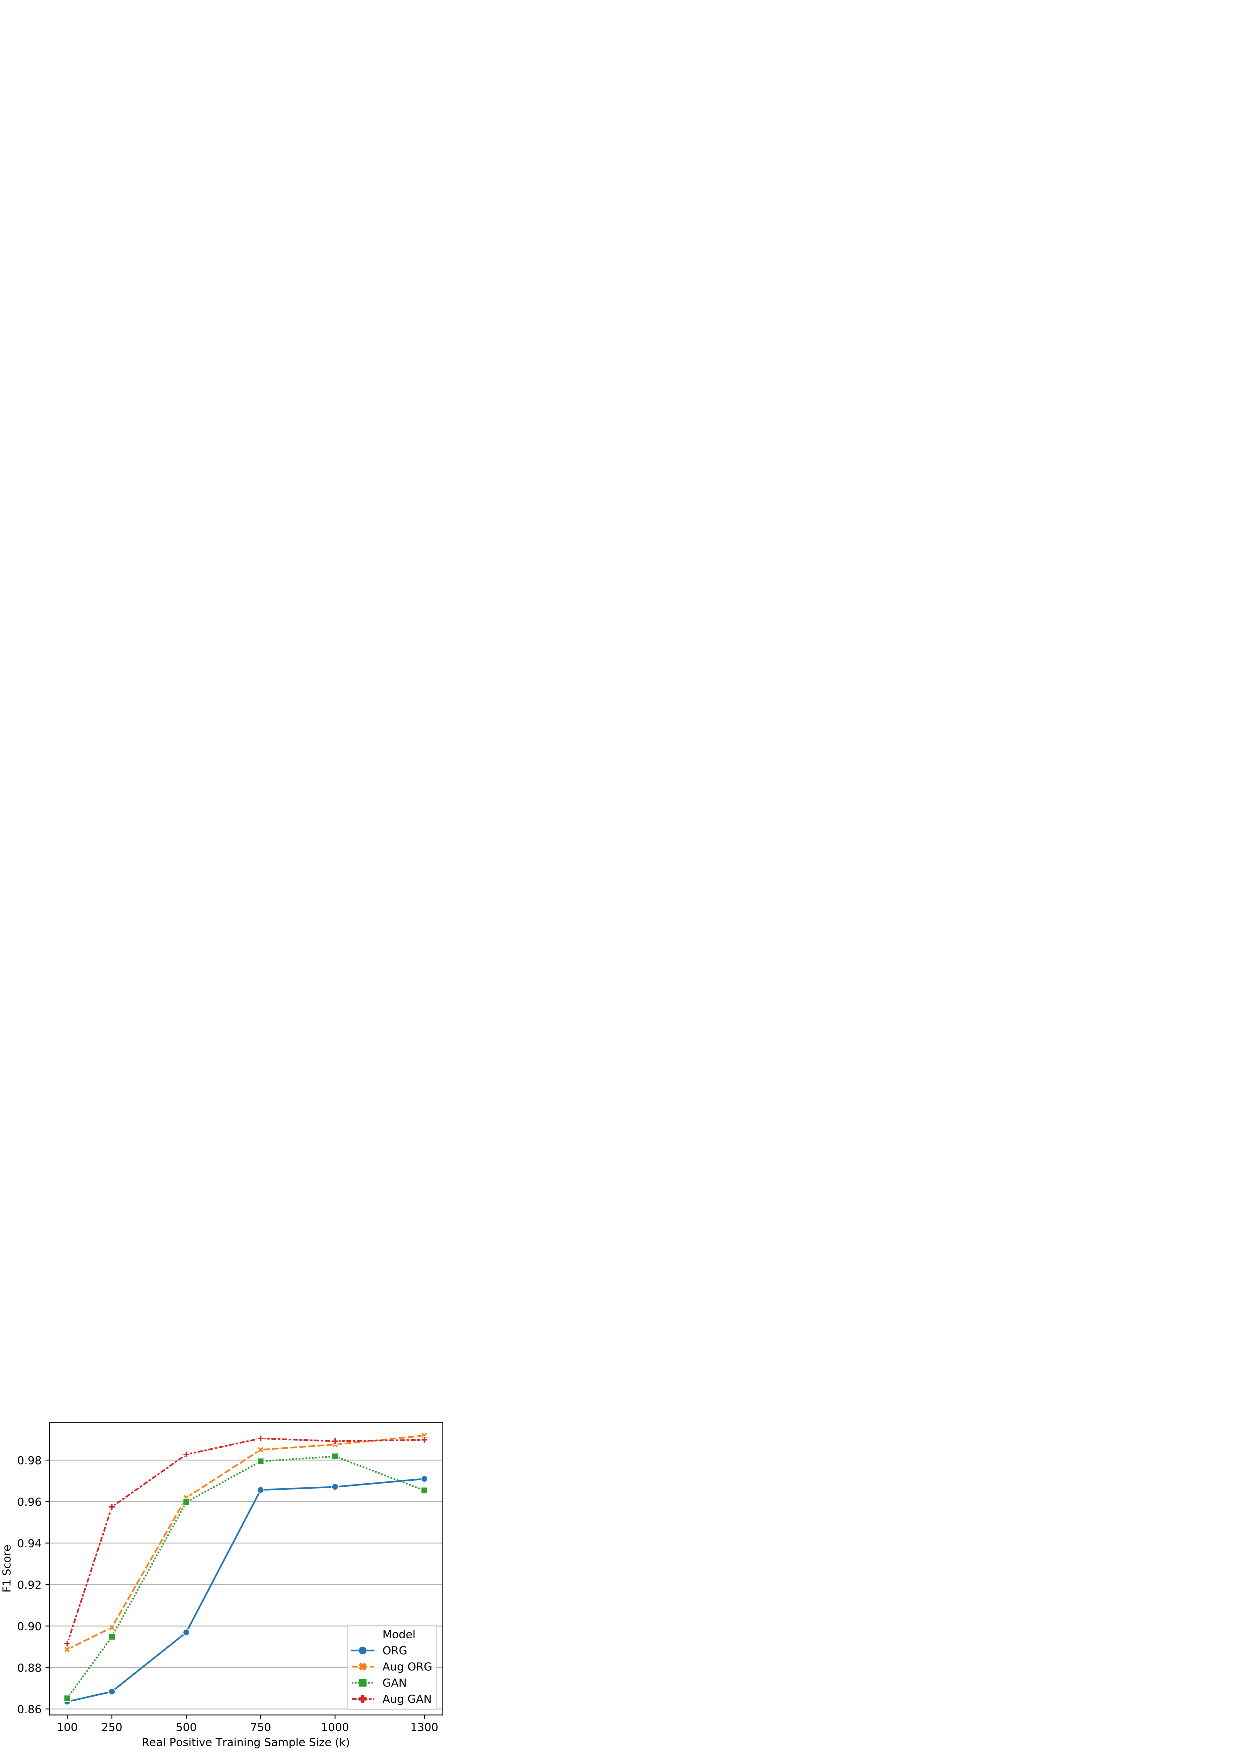
\includegraphics{figures/F1Score_allfolds.pdf}
    \caption{Examining F1 score as a function of the real minority training set size when adding $150\%$ generated images and keeping the same imbalance ratio 1:10. The horizontal axis represents the size of the training set of the positive class (mass lesions). ORG stands for the original dataset without any kind of augmentation, Aug ORG represents using the online random flipping on the original dataset, GAN means combining the original dataset with the generated images without augmentation, Aug GAN refers to online flipping applied on real (positive and negative) and DCGAN-generated images.}
    \label{fig:F1Score_augmentation}
\end{figure}

\begin{table*}[htp]
    \centering
        \caption{Area Uner the ROC Curve (AUC) for different modes and training sizes (k), the bold-faced values are the highest.}
    \begin{tabular}{|*{7}{c|}}
    \hline
         \multirow{2}{*}{Mode}   & \multicolumn{6}{|c|}{Training Size}  \\\cline{2-7}
                                    & 100 & 250 & 500 & 750 & 1000 & 1300 \\\hline
        ORG                         & 0.9836 & 0.9848 & 0.9896 & 0.999 & 0.9989 & 0.9989 \\\hline
        GAN                         & 0.9843 & 0.9902 & 0.9984 & 0.9997 & 0.9993 & 0.9987\\\hline
        Aug ORG                     & 0.9877 & 0.9896 & 0.9982 & \textbf{0.9998} & 0.9997 & 0.9999\\\hline
        Aug GAN                     & \textbf{0.9902} & \textbf{0.9984} & \textbf{0.9996} & 0.9990 & \textbf{0.9998} & \textbf{0.9999}\\\hline
    \end{tabular}

    \label{tab:auc_mass_aug}
\end{table*}

The green line represents the F1 score when adding synthetic images to the real ones (\textit{GAN} mode). The amount of added images differs from one case to another but always using $1.5 \times k$ as augmentation factor. Compared to the blue line, the green one shows faster improvements which shows that the generator has learned to unlock unseen images in the real distribution which help the classifier to distinguish lesions among normal tissue. At 100, as the plot shows, the improvements were fairly existing which is due to lack of enough samples for the DCGAN to learn the distribution of the real data. As this amount increases to 250, the improvement over ORG increases drastically pointing at a better-performing G. This improvement continued until 1000 where the classifier was no more starving for data. Surprisingly, at 1300, the DCGAN could generate samples visually similar to the real ones (see annex \ref{annex:5eachK} for an illustration of the effect of increasing the training set size on the generated images by DCGAN). However, this had a negative impact on the classification problem which might be due to overfitting. Additionally, the amount generated at 1300 ($1.5 \times 1300= 1950$) is the largest among all experiments which might have caused a drop in diversity. Moving on to the orange line representing \textit{Aug ORG} mode where online horizontal and vertical flipping with probability 0.5 was applied on every batch. Flipping was clearly outperforming \textit{GAN} due to lack of training images for the DCGAN as opposed to \textit{Aug ORG} where flipping algorithm is independent of any training. As the number of images, extrapolated images were increasing until 750 where the improvement reached a plateau as the classifier became less hungry to data. \textit{Aug ORG} and \textit{GAN} performed approximately equally in the region between the two extremes (100, 1300) with the difference becoming more obvious as k increases (see 750, 1000, and 1300). Finally, the red line represents \textit{Aug GAN} where the random flipping is applied online on the combined real and synthetically-generated images ending up with interpolation and extrapolation happening simultaneously. As can be seen in the figure, this mode outperformed all other modes. The amount of improvement was the largest at 250 and 500 as the classifier was in need for positive data, and became smaller as the classifier has seen enough samples at 750 and 1000). The last point at 1300 was less performing than \textit{Aug ORG} by a negligible amount. The Area Under the ROC Curve (AUC) was used as an additional metric to compare the performance with the different modes and training sizes. AUC values are reported in Table \ref{tab:auc_mass_aug}, the highlighted values are for the highest of the corresponding size. It can be easily seen from the table that \textit{Aug GAN} outperforms other modes where the highest improvement was for size 250 with 0.0136 over \textit{ORG} mode while the best improvement for \textit{Aug ORG} was for the same size by 0.0047 over \textit{ORG} mode.
Moreover, to analyse the distribution of the synthetically-generated images and to compare it to the distribution of the real images, t-SNE was used to reduce the dimensionality of the image space by moving to the 2D feature space. Figure \ref{fig:tSNE_real_fake} can be used to visualize the distributions for one case at $k=500$. The algorithm was run for a maximum number of iterations of 4000 and 250 as the perplexity. Similarly, Figure \ref{fig:tSNE_real_fake_tis} shows the distributions of real and fake masses along with normal tissue patches. It should be noted that this algorithm uses random initialization every time it is run, as a result, it might show different allocations for the samples in the figure for different runs. The input for the algorithm is the patches in the original space ($128 \times 128$) for both real and synthetic images.

\begin{figure*}[!htp]
\centering
\includegraphics[scale=1]{figures/tSNE_real_fake.pdf}
\caption{t-SNE analysis for real (red x) and generated (green circles) mass patches distributions, where X1 and X2 axes represent the first and second t-SNE components, respectively. }
\label{fig:tSNE_real_fake}
\end{figure*}

\subsection{Experimental Settings}
All models were built using Pytorch \footnote{code and trained generators are available at \url{https://github.com/Basel1991/Projects/tree/master/master_thesis}} package by \citet{pytorch} with the support of online augmentation.
Training a DCGAN then a classifier took on average two hours on NVIDIA TITAN X with 12 GB RAM using CUDA ver.9.0. The generator of the DCGAN had 5M parameters, while the discriminator had 8.9M. All these experiments were carried out at VICOROB lab at the University of Girona using a workstation running Linux Ubuntu 18.04. 


\section{Discussion}
\label{sec:discussion}
Regarding the results for lesion simulation, it has been shown that DCGAN could generate images that have considerable realism and diversity by training the DCGAN on a dataset that has a sufficient number of examples. The generator could capture the distribution of the real images ($p_{x}$) and generate samples that are sampled from $p_{gen}$ which is close to the original one.
Figure \ref{fig:real_or_fake} in Annex \ref{annex:ROF} can be used for a qualitative evaluation of the generated images. This figure shows one real batch of 64 mass lesions (top) along with the same number of synthetic ones (bottom). The size of the training set was 4536 mass and micro calcification lesions. For training details, see section \ref{sec:gan_training}. By comparing the top and the bottom batches, it can be seen that the generator has learned how to generate mass patches as well as mass accompanied with calcification (see real lesion (3,1) and fake (6,7)). Furthermore, this figure shows that the synthetic batch has reasonable diversity ending up in lesions with different shapes and contrast levels. Some of the shown synthetic examples seem to contain either mass only (see (1,5), (6,4), (7,3)), calcification only (see (6,2) and (8,2)), or a combination of mass and calcification (see (5,7), (4,2)).
While other works showed how much observers were fooled when distinguishing real among fake images, in this work we used FID in Figure \ref{fig:FID_lesion_simulation} as an objective evaluation method where the generated images had similar distributions of feature maps at the 2048-unit layer of Inception-v3. Some oscillations in FID values appear due to G being learning. As was mentioned in the talk of \citet{nips2016}, using different kernels between the discriminator and generator along with long training was useful to remove the checkerboard effect and improve the diversity. With respect to evaluating the simulated lesions, we proposed a framework where we train the DCGAN on different-size subsets of the mass dataset (inspired by the work of \citet{liver_aug}), the trained generators were used to generate synthetic lesions that were used to augment an imbalanced classification problem (normal tissue as the dominant negative class). It was shown that the improvement DCGAN introduced was related to the dataset size. The synthetic images did not improve the performance at a very early stage (very small dataset of 100 images), it did not cause any harm at this stage though. However, the improvement increased with the size of the training set. Moreover, and in line with the results of \citet{GAN_brain_aug}, the generated images did some harm for the classifier performance where the F1 score dropped when using the largest subset ($P_{1300}$) images for training, this suggests that there is a limit for the training set size to assure non-harmful GANs. Aligned with what was interestingly mentioned in \citet{GAN_brain_aug}, applying traditional flipping (online and random) method on the real and synthetic images (positive and negative classes) was powerful enough to make DCGAN-generated images helpful regardless the size of the training set (see the red line in Figure \ref{fig:F1Score_augmentation} for after augmentation and the green one for without augmentation). Additionally, we could show that using the real images only, increasing the size of the training set had a similar impact of enhancing the F1 score but with a much smaller rate with a tipping point where the improvement stops. The distribution of the generated images was analysed and compared to real ones in Figure \ref{fig:tSNE_real_fake} where it is clear that synthetic images support the distribution of the real ones by filling the gaps in a realistic way as opposed to naive methods which do the averaging of features as in SMOTE and its variations. Figure \ref{fig:tSNE_real_fake_tis} shows the distribution of real masses, synthetic masses, and normal tissue patches. This figure can show that by using synthetic images, the classifier can generalise more by seeing more examples sampled from the distribution of the minority class (a linear boundary can separate the two distributions). On the one hand, DCGAN could detect the features of the main distribution giving less support to outliers (see the arrow in Figure \ref{fig:tSNE_real_fake_tis}), traditional flipping, on the other hand, does not have the ability to distinguish between inliers (main distribution) and outliers (see the green distribution around the dotted arrow in Figure \ref{fig:tSNE_real_aug_tis} in Annex \ref{annex:t_SNE_real_aug_tis}) which can be linked to the improvement in \textit{Aug GAN} over all other methods in Figure \ref{fig:F1Score_augmentation} and Table \ref{tab:auc_mass_aug}. Matches, where at least one real and one synthetic samples align perfectly in the t-SNE space (see the solid arrow in Figure \ref{fig:tSNE_real_aug_tis}), are more common in traditional augmentation than in synthetic images due to the fact that the generator does not see the training images.


\begin{figure*}[htp]
\centering
\includegraphics[scale=1]{figures/tSNE_real_fake_tis_arrow.pdf}
\caption{t-SNE analysis for real (red cross) and generated (green circle) mass as well as normal tissue (purple triangle, the negative majority class) patches distributions, where X1 and X2 axes represent the first and second t-SNE components, respectively.}
\label{fig:tSNE_real_fake_tis}
\end{figure*}

\section{Conclusions}
\label{sec:conclusions}
In this study, we used a modified version of DCGAN to generate realistic mammographic lesions with dimensions $128 \times 128$ pixels that have acceptable diversity. To see the effect of using these synthetically-generated images in action, we simulated an environment where a dataset of mass lesions (as the positive class) and normal tissue (as the negative class) had to be classified with an imbalance ratio of 10. The classification performance was evaluated using F1 score and AUC at six different sizes of the positive dataset $(100, 250, 500, 750, 1000, 1300)$ keeping the same imbalance ratio, and validated using 3-fold cross validation. We could show that GANs-generated images when used along with online random horizontal then vertical reflection (named as \textit{Aug GAN}) were never harmful and could provide a significant improvement which is higher than when using GAN or flipping individually. This improvement was by the fact that at each size of the training set, \textit{AUG GAN} mode was higher than all other modes resulting in an F1 improvement of approximately $(2\%, 9\%, 8\%, 2\%, 2\%, 2\%)$ over using real images only and approximately $(0\%, 6\%, 2\%, 0.5\%, 0\%, 0\%)$ over using flipping only. Regarding AUC, we could achieve a max improvement of 0.013 over using real images only. Moreover, using synthetic images only as augmentation, there was a limitation at the very small or very large size of the training set where there was either no improvement or a drop in the performance, respectively, compared to real images only. Traditional image flipping augmentation did not suffer from such flaws even without the need for training but could not reach the same level of improvement that \textit{Aug GAN} offered. To sum up, GANs are a powerful tool that can be used to generate synthetic images to be used in a variety of applications including augmenting unbalanced classification problems and unlocking realistic unseen images. However, they have to be trained carefully and better be accompanied with traditional flipping augmentation. In the future, we plan to extend our work to see the effect of using the trained generators on supporting mass detection problems using a different dataset (INbreast). Generating larger patches or even complete mammograms can be explored as well. Furthermore, we are collaborating with radiologists from the Autonomous University of Barcelona to get realism evaluations of the generated mass patches.

\section{Acknowledgements}
Our great gratitude goes to Nvidia for supporting this work by a Titan X GPU.
I would like also to thank my supervisors for offering decent infrastructure and dataset as well as directing me to the target. I am in huge debt to Vicorob research institute, especially Mostafa Abubakr Salem (PhD) for his fruitful discussions and valuable suggestions regarding DCGAN training and testing. Special thanks go to Lavsen Dahal (MAIA) and Albert Garcia (PhD) for their continuous support and enlightening insights.

%\section*{References}
\bibliography{myThesisBibfile}

\section{Annex}
In these annexes, we show the outcome of four experiments. First, we present a real and a fake batches of 64 images each, where the fake ones were generated via a DCGAN trained on the complete training dataset (4536 mass + calcification). Second, a figure that shows the progress of training the DCGAN accompanied with the loss plot and a batch of 4 fake images enhancement during training. Third, we include t-SNE analysis for \textit{Aug ORG} showing real and augmented masses as well as normal tissue in the 2D feature space of t-SNE. Fourth and last, we show 25 random samples generated from six different generators trained on $(100, 250, 500, 750, 1000, 1300)$ images individually and we compare the quality and diversity. 

\subsection{A Real And A Fake Batch}
\label{annex:ROF}
In this section, 
using Figure \ref{fig:real_or_fake}, we show one real batch of 64 mass lesions (top) along with the same number of fake ones (bottom) generated by a generator that was trained on 4536 images (mass + calcification).

\subsection{GAN Training Progress}
\label{annex:GAN_progress}

Here we show the progress of G and D loss during training using the mass + calcification dataset of size 4536. The reflection on images realism and diversity is explored in Figure \ref{fig:GAN_prgoress} where it shows G and D average loss along with samples of 4 images generated from a fixed noise batch. By looking at the beginning of the plot (iteration 0), the loss of G starts high because it starts with random output which is relatively easy even for an inexperienced discriminator to realise that it is not real. In this case, the output of D for the fake input is very low (low realism probability). At iteration 0, D has just started to learn, however, the process of distinguishing real patches among real ones is considered easy, however, this becomes tougher when G starts learning. During iterations 0 to 20,000, G is learning from its mistakes by modifying the weights relatively to D output and competing with D which has a merely-constant average loss. A large drop of more than $70\%$ in FID is due to the large gradients of NS loss (see Figure \ref{fig:G_loss}). it can be seen from the difference in quality between the batches at epoch 140 and epoch 420 where the checkerboard effect was removed with an increase in realism and a decrease in FID. At iteration 25,000, D becomes almost professional and no more gets fooled by G output (D loss is monotonically decreasing), on the contrary, G loss starts increasing but keeps improving (see the image at epoch 700 where the lesions have been improved in terms of contrast and size). Iterations from 50K until 70K have lesser impact due to the learning rate here being too small compared to the early stages, still, this period had a subtle contribution to improvements in image diversity. By looking at FID values, it is clear that the decrease was exponentially decaying (along with the learning rate). At the end, the generator seems as it has lost the game by getting the loss settles at a relatively high value. It should be kept in mind here that the real label was randomly chosen every epoch which had the impact of the oscillations in the losses. The discriminator could keep detecting real images among fake ones ending up winning the game, this is fine as G had enough time to learn.

\subsection{t-SNE Analysis for Aug ORG}
\label{annex:t_SNE_real_aug_tis}

Figure \ref{fig:tSNE_real_aug_tis} shows the embeddings for 500 real mass patches, 750 with random flipping, and 5K normal tissue (negative majority).

\subsection{A Sample From Each $G_k$}
\label{annex:5eachK}
I this section, the aim is to evaluate subjectively the effect of increasing the training set size on the realism and diversity of the generated images. Figure \ref{fig:5eachK} shows six batches containing 25 images each, batches from top to bottom and left to right were generated by $G_{100}, G_{250}, G_{500}, G_{750}, G_{1000}, G_{1300}$ (see section \ref{sec:lesion_augmentation}). Starting with 100, this batch shows a low diversity (low recall) in lesions shapes with some similarity between lesions (see batch 100, (1,4) and (3,1), (3,3) and (4,3)). This suggests a mode collapse situation with the realism being not high. Moving on to batch 250, it is noticeable that lesions here have more contrast than before with some new shapes, however, there is still some patterns that are repeated between lesions (see batch 250 (1,1), (3,3) and (3,4)). Diversity keeps improving as well as realism when reaching to 500 and 750 where it is hard to detect such patterns. It can be seen that at 750 the generator has learned to sample lesions with more detailed architectures than before in batch 100. Batches 1000 and 1300 are where the generator starts to generate images that are hard to distinguish from real ones.

\begin{figure*}
    \centering
    \includegraphics[scale=.85]{figures/real_or_fake2.pdf}
    \caption{Two batches of real and fake images. The top one is the real batch while the bottom one is the fake one. Indices used here are of the shape (i,j), where i is the row index, j is the column index and the top left being (1,1). }
    \label{fig:real_or_fake}
\end{figure*}

\begin{figure*}
\centering
\includegraphics[scale=2]{figures/tSNE_real_aug_tis.pdf}
\caption{t-SNE distributions for real masses, flipped masses, and normal tissue patches. A red x represents a real mass patch, a green circle represents a flipped mass (horizontal, vertical, both, or none), purple triangles represent normal tissue patch. The dotted arrow points at an outlier while the solid one points at a match.}
\label{fig:tSNE_real_aug_tis}
\end{figure*}

\begin{figure*}
    \centering
    \includegraphics[scale=1, angle=0]{figures/GAN_progress2.pdf}
    
    \caption{GAN progress, showing 5 batches of generated images at different points in the training process, these images were taken from epochs 0, 140, 420, 700, and 990, where the input was fixed to four latent vectors. The horizontal axis is the training iterations, the vertical one is for DCGAN adversarial loss, see equations (1,2). FID values are approximated and provided for each case.}
    \label{fig:GAN_prgoress}
\end{figure*}


\begin{figure*}
    \centering
    \includegraphics{figures/5eachK.pdf}
    \caption{From top to bottom and left to right, 25 random samples generated from $G_k:\ k=\{100, 250, 500, 750, 1000, 1300\}$. This figure is to show the relationship between image quality and diversity, and number of training images for the DCGAN. Indices used here are of the shape (i,j), where i is the row index, j is the column index and the top left being (1,1).}
    \label{fig:5eachK}
\end{figure*}

\end{document} 
